\documentclass[english]{sareport}
% use the option peerreview for creating an anonymized version of your report
% E.g., \documentclass[english,peerreview]{sareport}

\usepackage[colorlinks, linkcolor=black, citecolor=black, urlcolor=black]{hyperref}


% Set all authors, if your group counts 2, set third author empty \authorthree{}
% Set the groupname as well
\authorone{Robin Haveneers (r0450702)}
\authortwo{Stef Verreydt (r0456110)}
\authorthree{Axel Lemmens (r0462440)}
\groupname{Haveneers-Verreydt-Lemmens}

\academicyear{2016--2017}

\casename{Shared Internet Of Things Infrastructure Platform}
\phasenumber{2a}
\phasename{ADD Application}


\begin{document}
\maketitle

\tableofcontents

\chapter{Introduction}\label{sec:introduction}
\todoinline{An introduction is not required, but if you include it, it should not be empty.}

\chapter{Attribute-driven design documentation}\label{sec:add}
\section{Decomposition 1: SIOTIP (M1, U2, UC6, UC8, UC13)}
\subsection{Module to decompose}
In this run we decompose \texttt{SIoTIP}.

\subsection{Selected architectural drivers}
The non-functional drivers for this decomposition are:

\begin{itemize}
	\item \emph{M1}: Integrate new sensor or actuator manufacturer
\end{itemize}
The related functional drivers are:

\begin{itemize}
	\item \emph{UC8}: Initialise a pluggable device
	\item \emph{UC9}: Configure pluggable device access rights
	\item \emph{UC10}: Consult and configure the topology
	\item \emph{UC13}: Configure pluggable device
\end{itemize}

\paragraph{Rationale}
M1 was chosen because it has high priority and because a lot of high priority usecases are linked to M1. \todo{Beter uitschrijven.}

\subsection{Architectural design}
\paragraph{GatewayFacade for M1}
M1 states that new types of sensor and actuator data should be transmitted to the online service. To accomodate for this, we first created a class \texttt{GatewayFacade} (representing the versasense gateway), which is responsible for relaying raw the sensor/actuator data to our system. This way, when a new peripheral (sensor/actuator) connects, the \texttt{GatewayFacade} automatically start to transmit the raw data of the new peripheral to our system.
\paragraph{Encapsulation of raw data for M1}
M1 also states that the new type of sensor data has to be processed by our system. To accomplish this we introduced a \texttt{PeripheralDB} wich stores all possible peripheral types with their corresponding conversion. This \texttt{PeripheralDB} offers an API to add new peripheral types. When a new peripheral type is introduced, it is the task of the manufracturer to add a new entry to the \texttt{PeripheralDB} including an identifier and a conversion function. We also implemented a \texttt{DataProcessingManager} which is responsible for receiving peripheral data from the gateway, processing and converting it to internal structures (using the \texttt{PeripheralDB}) and send it to the rest of our system. This increases semantic coherence by assigning only this specific task to the \texttt{DataProcessingManager}. By doing this, we ensure modifiability by making the \texttt{PeripheralDb} the only component that needs to be changed in order to accomodate for new peripheral types.
\paragraph{Intermediary for distributing data for M1}
Another requirement in M1 states that the peripheral data should be sent to the applications of the assigned customer organisations and should be stored. To solve this, we made a \texttt{DataDB} and a \texttt{AssignmentDB}. To former is responsible the data-records of all peripherals while the latter maps peripherals to customer organisations. In addition to these new structures we indroduced a \texttt{DataManager} to consult the \texttt{AssignmentDB} and send any incomming data (from the \texttt{DataProcessingManager}) to all applications that are allowed to access this peripheral data. It is also the responsibility of the \texttt{DataManager} to store the sensor data into the \texttt{DataDB}.

\paragraph{Incorporating new sensor}
M1 states that available applications can be updated to use any new pluggable devices. This requirement is met using the following structures. \texttt{Topology} is a data structure that keeps track of the installed sensors and actuators in the building. The \texttt{TopologyManager} provides an interface to the \texttt{ApplicationManager} only allowing acces to the peripherals it is assigned to in the \texttt{AssignmentDB}. Thus, adding a new pluggable device only impacts the \texttt{Topology} and thus available applications can be updated with ease to use the new pluggable devices. The \texttt{Application} uses the \texttt{Application Manager} interface to get an overview of the pluggable devices it can use. The \texttt{Application} can than specify, via the \texttt{Application Manager} from which pluggable device it wants to receive data.

\paragraph{Initialise pluggable device}
As stated in \emph{UC8} infrastructure owners must be able to initialize a new type of pluggable device. As mentioned before, this is why we introduced \texttt{PeripheralDB}. It offers an API to add new peripheral devices. The infrastructure owner is tasked to add a new entry to the \texttt{PeripheralDB} consisting of an identifier and the conversion method used for this pluggable, if any.

\paragraph{Configuring acces rights}
Furthermore, \emph{UC9} states that the infrastructure owner should be able to configure acces rights. For this we introduced the \texttt{AssignmentDB}. This database keeps track of which peripherals can be used by which customer organisations. If the infrastructure owner wants to configure the access rights, he is able to use the interface provided by this database to specify this relationship.

\paragraph{View detailed information about pluggable device}
When this new pluggable device is added to the system, the infrastructure owner wants to have the possibility to consult this device, as specified in \emph{UC10}. After initialising the device and configuring the acces rights, the new device is visible in the \texttt{Topology}. If the sensor is not yet in use, it is displayed on the side. In any case the infrastructure owner is able to view detailed information about the sensor using the interface provided by the \texttt{Topology}.


\subsubsection*{Alternatives considered}
\paragraph{Alternatives for \texttt{DataManager}}
An alternative we considered for using the \texttt{DataManager} would be to just have a direct relationship between the \texttt{ApplicationManager} and the \texttt{DataDB}. This way it would be the responsibility of the \texttt{ApplicationManager} of communcating with the \texttt{DataDB}. However, this way the \texttt{ApplicationManager} is able to view all the data in the \texttt{DataDB}, which is not desired. Moving the reponsibility of communicating with the \texttt{DataDB} seperates and localizes the responsibilities of each component even more. This approach was mentioned in our process of applying ADD, however it does not really add any advantages and thus was quickly rejected.
	
\paragraph{Alternatives for \texttt{AssigmentDB}}
A possible alternative for using the \texttt{AssignmentDB} was encapsulating the information directly in the topology which would also result in not having the need for a \texttt{TopologyManager}. However our approach lowers the coupling and in general makes the system more modifiable.
\todo{check this out}

\subsection{Instantiation and allocation of functionality}
\paragraph{Decomposition}
Figure \ref{fig:it1-cc_main} shows the components resulting from the decomposition in this run. 


\subparagraph{GatewayFacade}
Responsible for forwardig data from the pluggable devices to the system.

\subparagraph{DataProcessingManager}
Provides an interface for receiving data from the gatewa. Is responsible for looking up the appropriate conversion method in the \texttt{PeripheralDB} and applying it to the raw data. At last, this module is responsible for forwarding the processed data to the rest of the system.

\subparagraph{PeripheralDB}
Responsible for storing the different type of peripherals and their related conversion methods. Provides an interface for adding new types of peripherals along with the conversion methods and an interface to consult the database.

\subparagraph{DataManager}
This module is responsible for receiving processed data and storing it in the \texttt{DataDB}. It can consult the \texttt{AssignmentDB} to forward the data to the appropriate \texttt{ApplicationManager}.

\subparagraph{AssignmentDB}
Stores information about the relationships between peripherals and customer organizations. Provides an interface to look up this information as well as an interface to add new data to this database.

\subparagraph{ApplicationManager}
Responsible for keeping track of the sensors used by the corresponding application. It also provides an interface to configure sensors for a certain application. Is also responsible for forwarding the appropriate and correct information coming from the \texttt{DataManager} to the application.

\subparagraph{Application}
Receives appropriate data which it can use in its application logic.

\subparagraph{TopologyManager}
Provieds an interface to the \texttt{ApplicationManager} to consult the topology linked to the customer organisation who uses the \texttt{Application} linked with this \texttt{Application Manager}. Consults the \texttt{AssignmentDB} to see which peripherals are available to this \texttt{Application}.

\subparagraph{Topology}
Responsible for keeping track of peripherals distributed over a certain geographic location. Also keeps track of the relationship between avaiable sensors and provides an overview of sensors that are not yet avaialable. Also provides an interface to the infrastructure owner to configure new devices.
\begin{figure}[!htp]
	\centering
	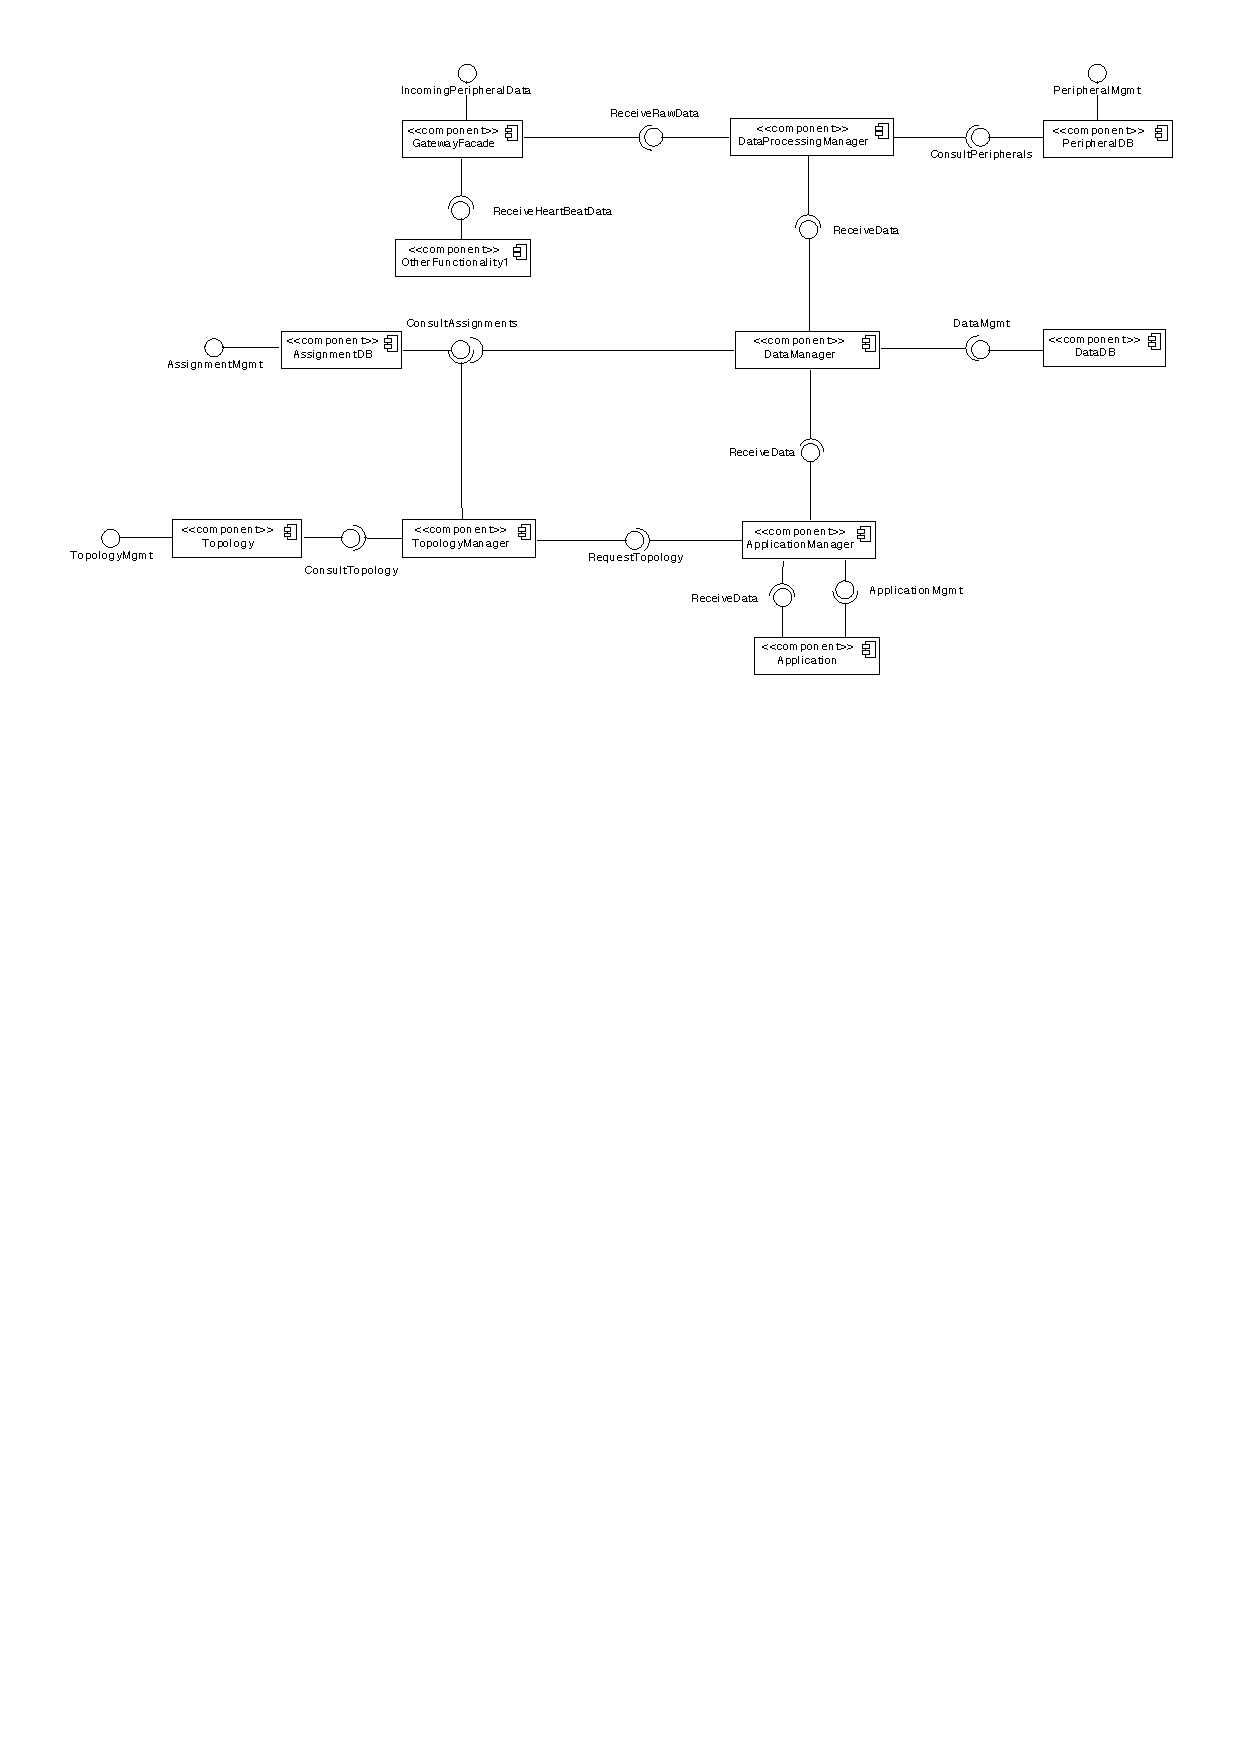
\includegraphics[width=0.8\textwidth]{component_diagram_1.pdf}
	%\missingfigure[figwidth=0.8\textwidth]{Component-and-connector diagram}
	\caption{Component-and-connector diagram of this decomposition.
	}\label{fig:it1-cc_main}
\end{figure}

\subsection{Verify and refine}
This section describes per component which (parts of) the remaining
requirements it is responsible for.

\paragraph{ApplicationManager}
\begin{itemize}
	\item \emph{Av2}: Application failure
\end{itemize}

\paragraph{DataDB}
\begin{itemize}
	\item \emph{P2}: Requests to the pluggable data database
\end{itemize}

\paragraph{GatewayFacade}
\begin{itemize}
	\item \emph{Av3b}: Pluggable device/mote failure detection
	\item \emph{UC11a}: Relay data from pluggable devices to the system
\end{itemize}

\paragraph{DataProcessingManager}
\begin{itemize}
	\item \emph{UC11b}: Convert raw data to a usable form and send it to the DataManager
\end{itemize}

\paragraph{DataManager}
\begin{itemize}
	\item \emph{UC11c}: Send data to all ApplicationManagers who belong to Applications which are authorized to use the sensor from which the data is sent.
	\item \emph{UC24b}: Process request for historical data and consult DataDB to retrieve data.
\end{itemize}

\paragraph{ApplicationManager}
\begin{itemize}
	\item \emph{Av2}: Application failure
	\item \emph{Av3b}: Redundancy when pluggable devices/motes fail \todoinline{Of is dit voor Application zelf?}
	\item \emph{U2b}: Out of the box working when sensors are available
	\item \emph{UC11d}: Send the data received from the DataManager to the Application only if the Application has indicated it needs the data.
	\item \emph{UC25}: Access topology and available devices
\end{itemize}

\paragraph{Application}
\begin{itemize}
	\item \emph{U1}: Application updates
	\item \emph{UC24a}: Send request for historical data
\end{itemize}

\paragraph{Topology}
\begin{itemize}
	\item \emph{U2a}: Edit topology when installing a new mote
\end{itemize}

\paragraph{OtherFunctionality1}
\begin{itemize}
	\item \emph{Av1}: Communication between SIoTIP gateway and Online Service
	\item \emph{P1}: Large number of users
	\item \emph{M2}: Big data analytics on pluggable data and/or application usage data
	\item \emph{U2c}: Reintroducing motes \todoinline{Voor Topology?} and mandatory end-user assignment
	\item \emph{UC1}: Register a customer organisation
	\item \emph{UC2}: Register an end-user
	\item \emph{UC3}: Unregister an end-user
	\item \emph{UC4}: Install mote
	\item \emph{UC5}: Uninstall mote
	\item \emph{UC6}: Insert a pluggable device into a mote
	\item \emph{UC7}: Remove a pluggable device from its mote
	\item \emph{UC12}: Perform actuation command
	\item \emph{UC14}: Send heartbeat
	\item \emph{UC15}: Send notification
	\item \emph{UC16}: Consult notification message
	\item \emph{UC17}: Activate an application
	\item \emph{UC18}: Check and deactivate applications
	\item \emph{UC19}: Subscribe to application
	\item \emph{UC20}: Unsubscribe from application
	\item \emph{UC21}: Send invoice
	\item \emph{UC22}: Upload an application
	\item \emph{UC23}: Consult application statistics
	\item \emph{UC26}: Send application command or message to external front-end
	\item \emph{UC27}: Receive application command or message from external frontend
	\item \emph{UC28}: Log in
	\item \emph{UC29}: Log out
\end{itemize}

\section{Decomposition 2: Module (drivers)}
\subsection{Module to decompose}
In this run we decompose \texttt{OtherFuntionality}.
\subsection{Selected architectural drivers}
The non-functional drivers for this decomposition are:

\begin{itemize}
	\item \emph{U2}: Easy installation
\end{itemize}

The related functional drivers are:

\begin{itemize}
	\item \emph{UC4}: Install mote
	\item \emph{UC5}: Uninstall mote
	\item \emph{UC6}: Insert a pluggable device into a mote
	\item \emph{UC7}: Remove a pluggable device from its mote
	\item \emph{UC14}: Send heartbeat
\end{itemize}

\paragraph{Rationale}
U2 was chosen because it has a high priority. UC4, UC5, UC6, UC7 are all concerned with the installation of pluggables and are therefore tightly linked with U2. The 4 first use cases all have high priority. UC14 is connected to U2 because it is an essential part of the easy installation and tighly connected to possibility to reintroduce previously connected nodes.
\subsection{Architectural design}
\paragraph{GatewayFacade for U2}
The \texttt{GatewayFacade} gets extended with the functionality of also transmitting the other types of messages, more specifcally the connection message and the heartbeat. Again, the \texttt{GatewayFacade} is reponsible for relaying this data to the Online Service where it can be processed and used in the necessary contexts. Whenever a mote is connected or disconnected a corresponding message is sent automatically. Whenever pluggables get plugged in a connected mote, this new pluggable will be included in the next heartbeat sent by the mote.

\paragraph{Installing new mote} 
As specified in U2, installing a new mote should not require any more configuration than adding it to the topology. This is met using the \texttt{GatewayFacade} and the \texttt{ConnectionManager}. Whenever a new mote is installed it emits a connection message. This connection message is forwarded and checked against the history of previously installed motes. Since it is a new mote no configuration can be retreived and the mote is added to the topology as an 'uninitiliased' device waiting to be configured by the infrastructure owner. Thus the only configuration required is the action performed by the infrastructure owner, which is possible via the interface \texttt{ToplogyMgmt} (as stated in the first decomposition). Configuring acces rights is not a necessity and thus after this the new mote is installed.

\paragraph{Reintroducing previously known mote - `Undo'ing the removal of the mote}
As stated in U2 it should be possible to reintroduce motes, i.e. if a previously known and configure mote gets reintroduced to the system, it should automatically retreive its configuration and reinstate the correct acces rights. This approach is based on the undo tactic and can be achieved by adhering to the memento pattern. Even though this is not really a undo, rollback scenario in the hard sense of the word, it is still tightly related. The memento object in this case is stored in the \texttt{DeviceHistoryDB}. In this case the originator is the mote itself and the origin of change comes from the \texttt{ConnectionManager} which handles the connection message and thus wishes to reinstate the previously configured mote. Thus, in this case, the \texttt{DeviceHistoryManager} will check the \texttt{DeviceHistoryDB} and will put back the necessary assignments in the \texttt{AssignmentDB} as explained in the first decomposition. Afterwards, the topology history gets passed to the \texttt{TopologyManger} and the device will be added to its last known position in the topology. No further configuration is required.
\subsection{Instantiation and allocation of functionality}
\paragraph{Decomposition}
Figure \ref{fig:it2-cc_main} shows the components resulting from the decomposition in this run. 

\subparagraph{ConnectionManager}
The main task of the \texttt{ConnectionManager} is to check for incoming connection and heartbeat messages. When a message arrives, it is the task of the \texttt{ConnectionManager} to forward it to the \texttt{DeviceHistoryManager} to check if the mote is reconnecting or if it is a new mote. In the former case, the \texttt{DeviceHistoryManager} returns the old configuration and this configuration is added to the topology via the \texttt{TopologyManager}. In the latter case, the new mote is temporarily added to the topology via the \texttt{TopologyManager}, awaiting further configuration by the infrastructure owner.

\subparagraph{DeviceHistoryManager}
It is the task of the \texttt{DeviceHistoryManager} to check if a connecting mote has already been connected in the past. If this is the case, it consults the \texttt{DeviceHistoryDB} to recover the mote's past configuration and assignments. Afterwards it will re-enter the old assignments into the \texttt{AssignmentDB} \footnote{Only if possible (if the state of the system is not drastically different).} and send the old topology-configuration to the \texttt{ConnectionManger}.

\subparagraph{DeviceHistoryDB}
Database that keeps past configurations and assignments of peripherals on disconnected motes to be able to easily restore to a previous state.

\subparagraph{ApplicationActivator}
When it receives a message from the \texttt{TopologyManager} (when the \texttt{Topology} is changed), it checks the \texttt{ApplicationActivationDB} if there is an application waiting on this new peripheral. When this is the case, the \texttt{ApplicationActivator} contacts the \texttt{ApplicationManager} to activate the waiting application.



\begin{figure}[!htp]
	\centering
	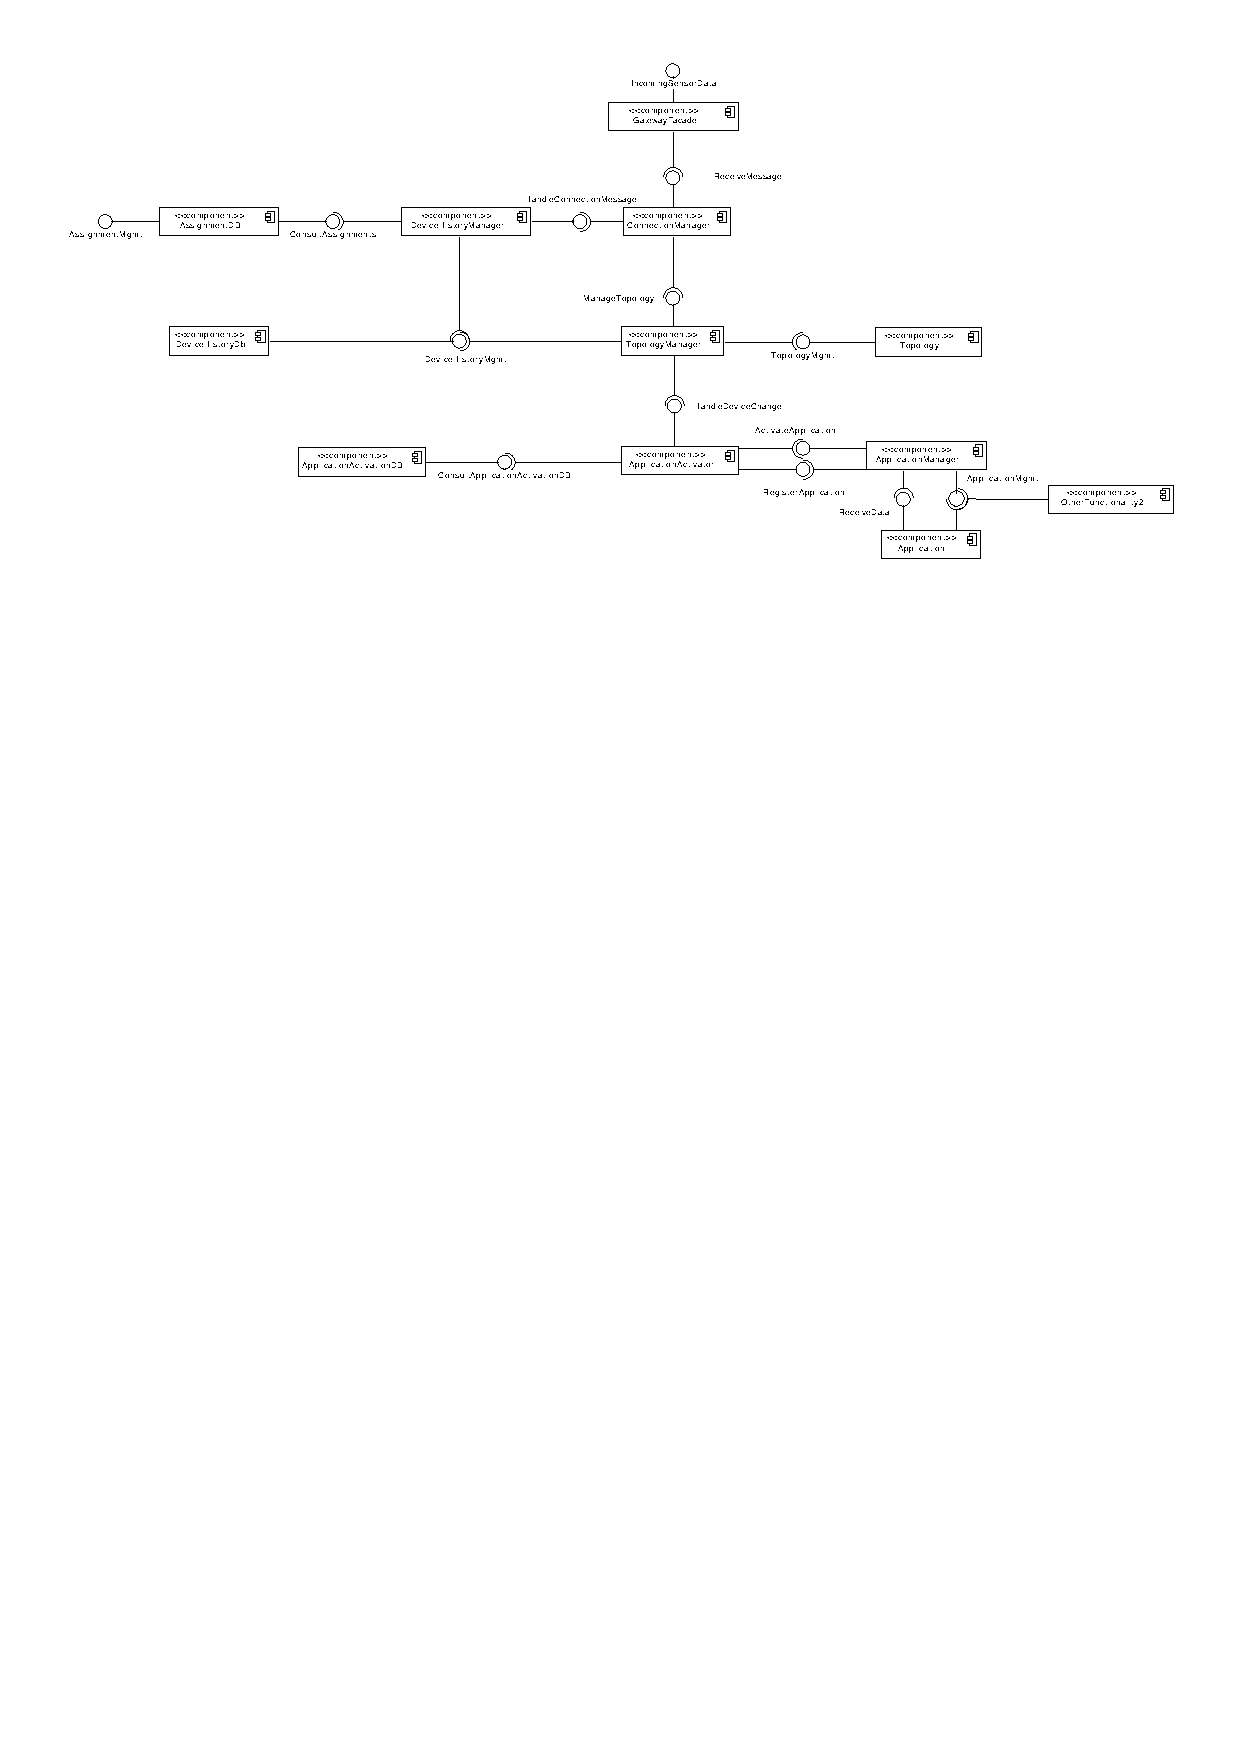
\includegraphics[width=0.8\textwidth]{component_diagram_2.pdf}
	%\missingfigure[figwidth=0.8\textwidth]{Component-and-connector diagram}
	\caption{Component-and-connector diagram of this decomposition.
	}\label{fig:it2-cc_main}
\end{figure}

\subsection{Interfaces for child modules}
\subsection{Data type definitions}
\subsection{Verify and refine}

\paragraph{ApplicationManager}
\begin{itemize}
	\item \emph{Av2}: Application failure
\end{itemize}

\paragraph{DataDB}
\begin{itemize}
	\item \emph{P2}: Requests to the pluggable data database
\end{itemize}

\paragraph{GatewayFacade}
\begin{itemize}
	\item \emph{UC11a}: Relay data from pluggable devices to the system
\end{itemize}

\paragraph{TopologyManager}
\begin{itemize}
	\item \emph{Av3b}: Pluggable device/mote failure detection
\end{itemize}

\paragraph{DataProcessingManager}
\begin{itemize}
	\item \emph{UC11b}: Convert raw data to a usable form and send it to the DataManager
\end{itemize}

\paragraph{DataManager}
\begin{itemize}
	\item \emph{UC11c}: Send data to all ApplicationManagers who belong to Applications which are authorized to use the sensor from which the data is sent.
	\item \emph{UC24b}: Process request for historical data and consult DataDB to retrieve data.
\end{itemize}

\paragraph{ApplicationManager}
\begin{itemize}
	\item \emph{Av2}: Application failure
	\item \emph{Av3b}: Redundancy when pluggable devices/motes fail \todoinline{Of is dit voor Application zelf?}
	\item \emph{U2b}: Out of the box working when sensors are available
	\item \emph{UC11d}: Send the data received from the DataManager to the Application only if the Application has indicated it needs the data.
	\item \emph{UC25}: Access topology and available devices
\end{itemize}

\paragraph{Application}
\begin{itemize}
	\item \emph{U1}: Application updates
	\item \emph{UC24a}: Send request for historical data
\end{itemize}

\paragraph{Topology}
\begin{itemize}
	\item \emph{U2a}: Edit topology when installing a new mote
\end{itemize}

\paragraph{OtherFunctionality1}
\begin{itemize}
	\item \emph{Av1}: Communication between SIoTIP gateway and Online Service
	\item \emph{P1}: Large number of users
	\item \emph{M2}: Big data analytics on pluggable data and/or application usage data
	\item \emph{U2c}: Reintroducing motes \todoinline{Voor Topology?} and mandatory end-user assignment
	\item \emph{UC1}: Register a customer organisation
	\item \emph{UC2}: Register an end-user
	\item \emph{UC3}: Unregister an end-user
	\item \emph{UC4}: Install mote
	\item \emph{UC5}: Uninstall mote
	\item \emph{UC6}: Insert a pluggable device into a mote
	\item \emph{UC7}: Remove a pluggable device from its mote
	\item \emph{UC12}: Perform actuation command
	\item \emph{UC14}: Send heartbeat
	\item \emph{UC15}: Send notification
	\item \emph{UC16}: Consult notification message
	\item \emph{UC17}: Activate an application
	\item \emph{UC18}: Check and deactivate applications
	\item \emph{UC19}: Subscribe to application
	\item \emph{UC20}: Unsubscribe from application
	\item \emph{UC21}: Send invoice
	\item \emph{UC22}: Upload an application
	\item \emph{UC23}: Consult application statistics
	\item \emph{UC26}: Send application command or message to external front-end
	\item \emph{UC27}: Receive application command or message from external frontend
	\item \emph{UC28}: Log in
	\item \emph{UC29}: Log out
\end{itemize}


\chapter{Resulting partial architecture}\label{sec:architecture}
This section provides an over of the architecture constructed through ADD\@.

\section{Context diagram}
This subsection discusses the context diagram.

\begin{figure}[!htp]
	\centering
	%\includegraphics[width=0.8\textwidth]{}
	\missingfigure[figwidth=0.8\textwidth]{Context diagram for component-and-
		connector view.}
	\caption{Context diagram for the component-and-connector view.
	}\label{fig:cc_context}
\end{figure}

\section{Component-and-connector view}
A short discussion of the component-and-connector view with the key
decompositions if any.

\begin{figure}[!htp]
	\centering
	%\includegraphics[width=0.8\textwidth]{}
	\missingfigure[figwidth=0.8\textwidth]{Component-and-connector diagram}
	\caption{Primary diagram for the component-and-connector view.
	}\label{fig:cc_main}
\end{figure}

\begin{figure}[!htp]
	\centering
	%\includegraphics[width=0.8\textwidth]{}
	\missingfigure[figwidth=0.8\textwidth]{Key decomposition}
	\caption{Decomposition of a component shown in Figure~\ref{fig:cc_main}
	}\label{fig:decomp_decomp1}
\end{figure}

\section{Deployment view}
A short discussion of the allocation of components to physical nodes based on a
context diagram and a deployment diagram.

\begin{figure}[!htp]
	\centering
	%\includegraphics[width=0.8\textwidth]{}
	\missingfigure[figwidth=0.8\textwidth]{Context diagram for the allocation
		view.}
	\caption{Context diagram for the allocation view.}\label{fig:depl_context}
\end{figure}

\begin{figure}[!htp]
	\centering
	%\includegraphics[width=0.8\textwidth]{}
	\missingfigure[figwidth=0.8\textwidth]{Deployment diagram}
	\caption{Primary diagram for the allocation view.}\label{fig:depl_main}
\end{figure}


\end{document}
